\chapter{Πολυκατηγορική Ταξινόμηση με τον GMl-ASLCS$_{0}$}
Η παρούσα εργασία ερείδεται επί της Διπλωματικής Εργασίας του Μίλτου Αλλαμανή ΧΧΧ, και, του Μανθάνοντος Συστήματος Ταξινομητών που ανέπτυξε. Το ΜαΣΤ αυτό, θα το ονομάσουμε, στα πλαίσια αυτής της εργασίας, GMl-ASLCS$_{\:0}$. Η ονομασία, εκ πρώτης όψης, προσομοιάζει στο ΜαΣΤ που εξετάσαμε στο προηγούμενο κεφάλαιο, τον AS-LCS. Στην πραγματικότητα, είναι η επέκτασή του, η προσαρμογή του, στον πολυκατηγορικό (Ml) χώρο, όπως ακριβώς και οι αλγόριθμοι που παρουσιάσαμε στην Εν. (\ref{subsec:algorithmAdjustment}). Ο GMl-ASLCS$_{\:0}$ κληρονομεί τις  βασικές λειτουργίες του πλαισίου λειτουργίας του AS-LCS, όπως τις παραμέτρους των κανόνων που εξελίσσει, και επεκτείνει άλλες, στο πολυκατηγορικό πεδίο. Η μηδενική υποσημείωση στην ονομασία του GMl-ASLCS$_{\:0}$ γίνεται για να καταδείξουμε ότι αυτό το σύστημα είναι η αφετηρία από όπου ξεκινάμε τη μελέτη, την ανάλυσή και την επέκτασή μας. Ο GMl-ASLCS$_{\:0}$ είναι η πρώτη προσέγγιση του προβλήματος της πολυκατηγορικής (ή πολυετικετικής) ταξινόμησης με μεθόδους της Εξελικτικής Υπολογιστικής και παρέχει τις πρώτες ενδείξεις πως η πολυκατηγορική ταξινόμηση είναι, όχι μόνο εφικτή, αλλά και το ίδιο αποτελεσματική με τους state of the art αλγορίθμους στο χώρο της πολυκατηγορικής ταξινόμησης. 
\\

Σε αυτό το κεφάλαιο: 

\begin{itemize}
\item παρουσιάζουμε τις αλλαγές που ήταν απαραίτητες να γίνουν στον AS-LCS ώστε να είναι σε θέση να ταξινομεί πολυκατηγορικά δείγματα, παρέχοντας έτσι το υπόβαθρο για την κατανόηση του GML-ASLCS$_{\:0}$ και του μοντέλου που αναπτύξαμε,
\item επισκεπτόμαστε, παράλληλα, τις βασικές συνιστώσες του GML-ASLCS$_{\:0}$, και,
\item μπαίνουμε σε μεγαλύτερο βάθος σε ορισμένες λειτουργίες του, ώστε να γίνουν κατανοητοί οι λόγοι για τους οποίους τις τροποποιούμε.
\end{itemize}

\section{Τροποποίηση της Αναπαράστασης Κανόνων}
Η Αναπαράσταση των Κανόνων που χρησιμοποιούνται από ένα ΜαΣΤ μονοκατηγορικής ταξινόμησης τροποποιείται, ώστε στο τμήμα συνθήκης τους να περιλαμβάνεται η απόφαση για πολλαπλές ετικέτες. Προτού αναφερθούμε στην αναπαράσταση των ετικετών, εξετάζουμε την αναπαράσταση του τμήματος συνθήκης για τους διαφορετικούς τύπους γνωρισμάτων: τα \emph{δυαδικά}, \emph{ονομαστικά}, και, \emph{πραγματικά} γνωρίσματα.

\subsection{Αναπαράσταση Δυαδικών Γνωρισμάτων}
Οι διαθέσιμες τιμές για ένα δυαδικό γνώρισμα είναι τρεις: \emph{Αληθής}, \emph{Ψευδής}, και \emph{Αδιαφορία}(\#). Ο χαρακτήρας \# συμβολίζει την αδιαφορία ενός κανόνα για την τιμή του αντίστοιχου γνωρίσματος στα δεδομένα εισόδου. Συνεπώς, ένας κανόνας της μορφής $111\# \Rightarrow 101$ καλύπτει \emph{δύο} δείγματα: το $1111 \Rightarrow 101$, και το $1110 \Rightarrow 101$. Λόγω της ύπαρξης τριών πιθανών καταστάσεων για την τιμή ενός δυαδικού γνωρίσματος, χρησιμοποιούνται δύο δυαδικά ψηφία για την αναπαράσταση της. Ένα δυφίο, το λεγόμενο \emph{Ψηφίο Ενεργοποίησης}, καθιστά το \emph{Ψηφίο Τιμής} σχετικό ή άσχετο: εάν το Ψηφίο Ενεργοποίησης έχει τιμή μηδέν, ο κανόνας που το περιέχει αδιαφορεί για το συγκεκριμένο γνώρισμα. Σε αντίθετη περίπτωση, η τιμή του γνωρίσματος ταυτίζεται με την τιμή  του Ψηφίου Τιμής.

$$ \overbrace{
\underbrace{b_{1}}_\text{ψηφίο ενεργοποίησης} \:
\underbrace{b_{0}}_\text{ψηφίο τιμής}}
^\text{Συνθήκη Δυαδικού Γνωρίσματος}$$

\subsection{Αναπαράσταση Ονομαστικών Γνωρισμάτων}
Η αναπαράσταση ονομαστικών γνωρισμάτων αποτελεί γενίκευση αυτής των δυαδικών. Περιέχει και αυτή ένα ψηφίο ενεργοποίησης, και για την αναπαράσταση των $n$ τιμών ενός ονομαστικού γνωρίσματος χρησιμοποιεί μία δυαδική μάσκα $n$ δυφίων. Μία μη μηδενική τιμή ενός από αυτά τα δυφία υποδηλώνει την αντίστοιχη τιμή του ονομαστικού γνωρίσματος. Όταν η μάσκα ενεργοποίησης εφαρμοσθεί σε ένα δείγμα και προκύψει τιμή διάφορη του μηδενός, τότε ο κανόνας καλύπτει το δείγμα για τη συγκεκριμένη συνθήκη.

$$ \overbrace{
\underbrace{b_{n}}_\text{Ψηφίο Ενεργοποίησης}
\underbrace{b_{n-1}b_{n-2}
\dots b_{1}b_{0}}_\text{μάσκα τιμών}
}^\text{Συνθήκη Ονομαστικού Γνωρίσματος}$$

\subsection{Αναπαράσταση Συνθηκών Πραγματικών Γνωρισμάτων}
Για την αναπαράσταση συνθηκών πραγματικών γνωρισμάτων επιλέχθηκε η αναπαράσταση \emph{διαστήματος τιμών}, η οποία ορίζει ένα διάστημα επιτρεπτών τιμών για το γνώρισμα στο οποίο αναφέρονται, καθιστώντας εφικτή και τη δημιουργία μονόπλευρων ανισοτήτων. Επιπρόσθετα, επιλέχτηκε η αναπαράσταση θέσης για την κωδικοποίηση των εμπλεκομένων πραγματικών αριθμών. Στην αναπαράσταση θέσης, επειδή είναι εκ των προτέρων γνωστές η μέγιστη και η ελάχιστη τιμή ενός γνωρίσματος, κβαντίζονται οι ενδιάμεσες τιμές και αντιστοιχίζονται στις προκύπτουσες στάθμες τα δυαδικά ψηφία που χρησιμοποιούνται για την αναπαράσταση ενός αριθμού. Με αυτόν τον τρόπο, χρησιμοποιούνται, μεν, όλα τα διαθέσιμα δυαδικά ψηφία χωρίς να υπάρχει η ανάγκη για διόρθωση, καθίσταται, δε, πολυπλοκότερος ο υπολογισμός του πραγματικού αριθμού στον οποίο αντιστοιχεί το γονίδιο:
\\

\begin{equation} 
x_{i}=min_{i}+\frac{int(gene_{i})}{2^b}(max_{i} - min_{i}) 
\end{equation}  
\\

όπου $x_{i}$ η πραγματική τιμή του γνωρίσματος $i$, $max_{i}$ και $min_{i}$ οι καθολικές μέγιστες και αντίστοιχα ελάχιστες τιμές του γνωρίσματος, $b$ ο αριθμός των δυαδικών ψηφίων που χρησιμοποιήθηκαν στην αναπαράσταση και $gene_{i}$ η δυαδική αναπαράσταση του γονιδίου. Να σημειωθεί ότι το $b$ είναι μια παράμετρος με την οποία μπορεί να ελεγχθεί η διακριτική ικανότητα του κανόνα. Μεγαλύτερες τιμές του $b$, οδηγούν σε μεγαλύτερη ακρίβεια, με κόστος την αύξηση του μεγέθους του γονιδίου. Συνολικά, με βάση την αναπαράσταση των πραγματικών τιμών που επιλέχθηκε, για $2^{k}$ στάθμες κβαντισμού, η δομή των συνθηκών πραγματικών γνωρισμάτων μπορεί να αποδοθεί σχηματικά ως εξής:
\\

$$ \overbrace{
\underbrace{b_{2k}}_\text{ψηφίο ενεργοποίησης}
\underbrace{b_{2k-1}b_{2k-2}
\dots b_{k+1}b_{k}}_\text{άνω όριο}
\underbrace{b_{k-1}b_{k-2
}\dots b_1b_0}_\text{κάτω όριο}}
^\text{Συνθήκη Πραγμ. Γνωρισμάτων με Αναπαράσταση Διαστήματος Τιμών}$$
\\

\subsection{Αναπαράσταση του Τμήματος Απόφασης}
Η αναπαράσταση των κατηγοριών - ετικετών είναι σαφέστατα κρίσιμης σημασίας. Στην κατηγοριοποίηση μίας κατηγορίας, η αναπαράσταση είναι κάτι το τετριμμένο: οι πιθανές τιμές της μοναδικής ετικέτας - απόφασης αναπαριστώνται ως φυσικοί αριθμοί, και ενσωματώνονται στην αναπαράσταση του γονιδίου ως δυαδικοί. Στην πολυκατηγορική ταξινόμηση υπάρχει μεγάλος χώρος για εναλλακτικές προσεγγίσεις - από την \emph{αναπαράσταση μόνο μίας ετικέτας}, όπως στην απλή κατηγοριοποίηση, μέχρι τη \emph{σαφή αναπαράσταση όλων των ετικετών}, και την \emph{αναπαράσταση ετικετών με αδιαφορίες}. Τελικά, επιλέχθηκε η τελευταία, καθώς, η πρώτη προσεγγίζει τη μέθοδο μετασχηματισμού προβλημάτων $BR$, ή αν αναπαρασταθούν όλες οι ετικέτες στο ίδιο ΜαΣΤ, τη μέθοδο $RT$. Η δεύτερη, έχει ως αποτέλεσμα την παραγωγή εξαιρετικά συγκεκριμένων κανόνων, που αποφασίζουν πάντοτε υπέρ ή κατά της ταξινόμησης σε μία κατηγορία, αυξάνοντας το χώρο αναζήτησης των πιθανών καταστάσεων απόφασης, δυσκολεύοντας τον Γενετικό Αλγόριθμο να συγκλίνει, ειδικά σε περιπτώσεις χαλαρής εξάρτησης μεταξύ των ετικετών. 
\\
Η αναπαράσταση ετικετών με αδιαφορίες προσομοιάζει στην αναπαράσταση συνθηκών δυαδικών γνωρισμάτων. Κάθε κανόνας διαθέτει τη δυνατότητα να αποφασίσει υπέρ ή κατά της ταξινόμησης σε μία δεδομένη ετικέτα, ή ακόμα να απέχει από τη διαδικασία απόφασης, αδιαφορώντας. Για $\abs{L}$ αριθμό ετικετών, το τμήμα απόφασης των κανόνων παίρνει τη μορφή:
\\

\begin{center}
\begin{tikzpicture}
\node[align=center,draw,shape=rectangle split,rectangle split horizontal,rectangle split parts=4, text width=2cm] (A) at (0,0) 
{$a_{0}l_{0}$
\nodepart{two}$a_{1}l_{1}$
\nodepart{three}$\ldots$
\nodepart{four}$a_{\abs{L} - 1}l_{\abs{L} - 1}$};
\end{tikzpicture}
\end{center}



όπου $a_{i}$ το ψηφίο ενεργοποίησης και $l_{i}$ το δυφίο απόφασης για την ετικέτα $i$.
Σε αντίθεση με τη σαφή αναπαράσταση, οι βέλτιστοι κανόνες ορίζονται ως αυτοί με τη μέγιστη δυνατή κάλυψη και ταυτόχρονα το ειδικότερο δυνατό τμήμα απόφασης. Το σύστημα, λοιπόν, θα πρέπει να ισορροπήσει την εξερεύνηση του μεταξύ κανόνων γενικών, με πολλές αδιαφορίες στο τμήμα απόφασής τους, και κανόνων ειδικών με ελάχιστες αδιαφορίες. Ένας αποτελεσματικός τρόπος ώθησης του συστήματος προς αυτή την κατεύθυνση είναι η απαγόρευση συμμετοχής στα σχηματιζόμενα ανά ετικέτα Correct Sets (η τροποποίηση της διαδικασίας ενημέρωσης και ο μηχανισμός ώθησης αναλύονται στην Εν. \ref{sec:multiLabelUpdate}) των κανόνων που αδιαφορούν για κάθε δεδομένη ετικέτα για την οποία σχηματίζεται το αντίστοιχο Correct Set. 
\\
Η χρήση της αναπαράστασης με αδιαφορίες μπορεί, ανάλογα με το πρόβλημα, να οδηγήσει σε μοντέλα που προσεγγίζουν όλο το φάσμα που ορίζεται από τις ακραίες περιπτώσεις των μετασχηματισμών $BR$ (που χρησιμοποιεί μία ετικέτα) και $LC$ (που χρησιμοποιεί όλους τους πιθανούς συνδυασμούς ετικετών). Ωστόσο, στα μειονεκτήματα αυτού του τρόπου αναπαράστασης θα πρέπει να προσμετρηθεί η πολυπλοκότητα που εισάγει στη διαδικασία εξερεύνησης (βλ. \ref{sec:multiLabelExploration}) και τις στρατηγικές συμπερασμού (βλ. \ref{sec:multiLabelInference}). Τέλος, το γράμμα $G$ στην ονομασία GMlAS-LCS$_{\:0}$ αναφέρεται σε ακριβώς αυτή την αναπαράσταση των ετικετών: την αναπαράσταση με σαφή χρήση αδιαφοριών.


\section{Συνιστώσα Εξερεύνησης}
\label{sec:multiLabelExploration}
Η συνιστώσα ενημέρωσης αποτελείται, όπως και στην απλή κατηγοριοποίηση, από δύο τμήματα: το Γενετικό Αλγόριθμο και το τμήμα Κάλυψης. Ο Γενετικός Αλγόριθμος δεν επιδέχεται βαθιών αλλαγών, καθώς μεταχειρίζεται απλώς χρωμοσώματα, και αδιαφορεί για την αναπαράσταση του υποκείμενου προβλήματος. Συνεπώς μπορεί να διατηρηθεί χωρίς δομικές τροποποιήσεις. 

\subsection{Γενετικός Αλγόριθμος}
\label{subsec:gmlaslcs0GA}
Ο GMl-ASLCS$_{\:0}$ χρησιμοποιεί επιλογή ρουλέτας (βλ. \ref{subsec:rouletteWheelSelection}), επιλέγοντας τον κανόνα $i$ για να αποτελέσει υποψήφιο γονέα με πιθανότητα
\footnote{Ο αναγνώστης θα προσέξει τη διαφορά της χρήσης της πληθικότητας του κανόνα ανάμεσα στην παραπάνω εξίσωση και την  Εξ. \ref{eq:rouletteWheelSelectionWithoutNumerosity}. Ο κανόνας στου οποίου την πιθανότητα επιλογής αναφερόμαστε, είναι ένας \emph{μακροκανόνας}, και αυτή θα είναι η αναφορά της λέξης \emph{κανόνας} από εδώ και στο εξής. Για την αναφορά σε έναν συγκεκριμένο κανόνα, δηλαδή έναν κανόνα που συνολικά είναι μέρος ενός μακροκανόνα, θα χρησιμοποιούμε τον όρο \emph{μικρο-κανόνας}.}

\begin{equation}
P(i) = \frac{num(i) \cdot fitness(i)}{\sum\limits_{j=1}^n \big(num(j) \cdot fitness(j)\big)}
\end{equation}
όπου $n = \sum macroclassifiers$, δηλαδή το σύνολο του αριθμού των κανόνων του πληθυσμού.

Στην παραπάνω εξίσωση, το μέγεθος $fitness$ αποτελεί την καταλληλότητα που έχει υποστεί έκπτωση-βασισμένη-στην-εμπειρία (experience-based fitness discount), ακολουθώντας την πρακτική της βιβλιογραφίας:
\\

\begin{equation}
\label{eq:fitnessDiscount}
fitness(i) = \left\{
\begin{array}{ c l }
\displaystyle 0, 					& experience(i) < \theta_{exp}
\\
\displaystyle (accuracy(i))^{\nu}, 	& $αλλού$
\end{array}
\right.
\end{equation}
\\


Στην ουσία πρόκειται για καθυστέρηση στην εμπιστοσύνη τους συστήματος προς του κανόνες, εξυπηρετώντας, εν μέρει
\footnote{Ακριβέστερα, αποτρέπει τη συμμετοχή υπερ-γενικών κανόνων στην εξελικτική διαδικασία, έως ότου η εμπειρία τους ξεπεράσει το κατώφλι $\theta_{exp}$}
την αναπαραγωγή γενικών κανόνων, καθώς, η εμπειρία είναι ένα μέτρο της γενικότητας ενός κανόνα, κυρίως στις πρώτες επαναλήψεις της εκπαίδευσης, πάντα σε σεβασμό προς την ορθότητά τους, . Όσο πιο γενικός ένας κανόνας, τόσα περισσότερα δείγματα καλύπτει, και, άρα, σε τόσα περισσότερα $[M]$ συμμετέχει. Καθώς η εμπειρία ενός κανόνα αυξάνει κατά ένα σε κάθε $[M]$ που συμμετέχει, όσο πιο γενικός είναι, τόσο πιο γρήγορα θα ξεπεράσει το κατώφλι εμπειρίας $\theta_{exp}$, άρα τόσο πιο γρήγορα θα του ανατεθεί μία μη μηδενική πιθανότητα επιλογής από το Γενετικό Αλγόριθμο. Ένας ακόμα λόγος που συνηγορεί στη χρήση έκπτωσης βασισμένη στην εμπειρία είναι η απαίτηση μας ώστε το σύστημα να αποφασίζει για την επιλογή ενός κανόνα για αναπαραγωγή, βασισμένο σε μία πιο διαπιστωμένη του εικόνα για τον κανόνα. Εν γένει, θα μπορούσαμε να παρατηρήσουμε το φαινόμενο ένας κανόνας να μπορεί να ταξινομεί ορθά ένα από τα πρώτα δείγματα που καλύπτει, αλλά να αποτυγχάνει πλήρως να ταξινομήσει μεταγενέστερα. Αν το σύστημα τον εμπιστευόταν πλήρως εξαρχής, θα αναπαρήγαγε την αποτυχία του κανόνα στην ταξινόμηση εκείνων ακριβώς των δειγμάτων που θα προκαλούσαν τη μείωση της ορθότητάς του, απομακρύνοντας έτσι την αρχική μας απαίτηση για αναπαραγωγή βασισμένη στην ορθότητα.

Μετά την επιλογή δύο κανόνων-γονέων, έστω $A$ και $B$, στην ουσία εφαρμόζεται διασταύρωση ενός σημείου για την παραγωγή \emph{δύο} απογόνων. Το σημείο στο οποίο θα γίνει διασταύρωση επιλέγεται ξεχωριστά για τον κάθε απόγονο, ψευδο-τυχαία, και χωρίς βλάβη της γενικότητας έχει διαφορετική τιμή για τον καθένα. Μετά τον καθορισμό του σημείου διασταύρωσης, ο απόγονος $A$ προκύπτει από τη σύνθεση του χρωμοσώματος του γονέα $A$ μέχρι το σημείο διασταύρωσης και του γονέα $B$ από το σημείο διασταύρωσης μέχρι το τέλος του χρωμοσώματος του. Αντίστοιχα, ο απόγονος $B$ προκύπτει από τη σύνθεση του χρωμοσώματος του γονέα $B$ μέχρι το σημείο διασταύρωσης και του γονέα $A$ από το σημείο διασταύρωσης μέχρι το τέλος του χρωμοσώματος του.

Η διαδικασία απεικονίζεται στο σχήμα \ref{fig:singlePointCrossoverOffsprings}, με ανοιχτό χρώμα για τα γνωρίσματα, σκούρο για τις ετικέτες και $X$ να υποδηλώνει το εκάστοτε σημείο διασταύρωσης.


\begin{figure}[h!]
\centering
  \begin{center}
Γονέας$A$:\hspace*{5mm}
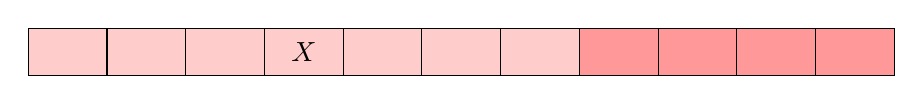
\begin{tikzpicture}[x=1cm, y=0cm, node distance=0cm,outer sep = 0pt]
\tikzstyle{gene}=[rectangle,draw,minimum width=1cm,minimum height=0.6cm]
\tikzstyle{aa}=[gene,fill=red!20]
\tikzstyle{al}=[gene,fill=red!40]

\node[aa] at (1,0) {};
\node[aa] at (2,0) {};
\node[aa] at (3,0) {};
\node[aa] at (4,0) {$X$};
\node[aa] at (5,0) {};
\node[aa] at (6,0) {};
\node[aa] at (7,0) {};
\node[al] at (8,0) {};
\node[al] at (9,0) {};
\node[al] at (10,0) {};
\node[al] at (11,0) {};

\end{tikzpicture}
\end{center}


\begin{center}
Απόγονος$A$:
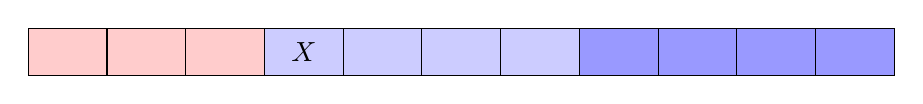
\begin{tikzpicture}[x=1cm, y=0cm, node distance=0cm,outer sep = 0pt]
\tikzstyle{gene}=[rectangle,draw,minimum width=1cm,minimum height=0.6cm]
\tikzstyle{aa}=[gene,fill=red!20]
\tikzstyle{al}=[gene,fill=red!40]
\tikzstyle{ba}=[gene,fill=blue!20]
\tikzstyle{bl}=[gene,fill=blue!40]

\node[aa] at (1,0) {};
\node[aa] at (2,0) {};
\node[aa] at (3,0) {};
\node[ba] at (4,0) {$X$};
\node[ba] at (5,0) {};
\node[ba] at (6,0) {};
\node[ba] at (7,0) {};
\node[bl] at (8,0) {};
\node[bl] at (9,0) {};
\node[bl] at (10,0) {};
\node[bl] at (11,0) {};

\end{tikzpicture}
\end{center}


\begin{center}
Γονέας$B$:\hspace*{5mm}
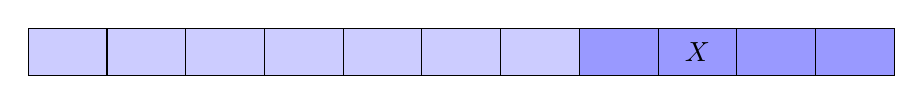
\begin{tikzpicture}[x=1cm, y=0cm, node distance=0cm, outer sep = 0pt]
\tikzstyle{gene}=[rectangle,draw,minimum width=1cm,minimum height=0.6cm]
\tikzstyle{ba}=[gene,fill=blue!20]
\tikzstyle{bl}=[gene,fill=blue!40]

\node[ba] at (1,0) {};
\node[ba] at (2,0) {};
\node[ba] at (3,0) {};
\node[ba] at (4,0) {};
\node[ba] at (5,0) {};
\node[ba] at (6,0) {};
\node[ba] at (7,0) {};
\node[bl] at (8,0) {};
\node[bl] at (9,0) {$X$};
\node[bl] at (10,0) {};
\node[bl] at (11,0) {};

\end{tikzpicture}
\end{center}





\begin{center}
Απόγονος$B$:
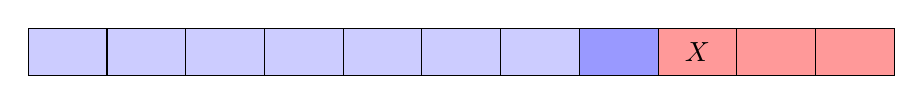
\begin{tikzpicture}[x=1cm, y=0cm, node distance=0cm, outer sep = 0pt]
\tikzstyle{gene}=[rectangle,draw,minimum width=1cm,minimum height=0.6cm]
\tikzstyle{ba}=[gene,fill=blue!20]
\tikzstyle{bl}=[gene,fill=blue!40]
\tikzstyle{aa}=[gene,fill=red!20]
\tikzstyle{al}=[gene,fill=red!40]

\node[ba] at (1,0) {};
\node[ba] at (2,0) {};
\node[ba] at (3,0) {};
\node[ba] at (4,0) {};
\node[ba] at (5,0) {};
\node[ba] at (6,0) {};
\node[ba] at (7,0) {};
\node[bl] at (8,0) {};
\node[al] at (9,0) {$X$};
\node[al] at (10,0) {};
\node[al] at (11,0) {};

\end{tikzpicture}
\end{center}
  \caption{Διαδικασία Διασταύρωσης στον GMl-ASLCS$_{\:0}$}
  \label{fig:singlePointCrossoverOffsprings}
\end{figure}

Ο τελεστής της διασταύρωσης εφαρμόζεται με πιθανότητα $X = 0.8$. Σε περίπτωση απόφασης μη διασταύρωσης, οι απόγονοι βγαίνουν αλώβητοι από τη διαδικασία της διασταύρωσης, ως κλώνοι των γονέων τους. Σε κάθε περίπτωση, στη συνέχεια, και κατά τα γνωστά, εφαρμόζεται ο τελεστής της \emph{ομοιόμορφης μετάλλαξης}, δηλαδή κάθε γνώρισμα και ετικέτα υπόκειται ξεχωριστά σε μετάλλαξη, με πιθανότητα $\mu = 0.04$. Οι απόγονοι, προτού εισαχθούν στον πληθυσμό, ελέγχονται για υπαγωγή (subsumption) με το σύνολο των κανόνων. Εάν υπάρχει κάποιος κανόνας αρκούντως έμπειρος, τουλάχιστον ίδιος ή γενικότερος στο τμήμα της συνθήκης και, ταυτόχρονα, τουλάχιστον ίδιος ή ειδικότερος στο τμήμα της απόφασης, ο νέος κανόνας δεν εισάγεται στον πληθυσμό, αλλά αφομοιώνεται από αυτόν, αυξάνοντας την πληθικότητα του κατά ένα. Σε αντίθετη περίπτωση ο κανόνας-απόγονος εισάγεται απευθείας στον πληθυσμό ως αυτοτελής κανόνας, χωρίς κάποια περαιτέρω διαδικασία.
\\

\paragraph{Λειτουργία Διαγραφής}
Όπως και στα σχήματα αναπαραγωγής των UCS και AS-LCS, έτσι και εδώ, το σύστημα εξελίσσει ένα σύνολο από κανόνες του οποίου ο συνολικός αριθμός, δηλαδή το άθροισμα των πληθικοτήτων των κανόνων, παραμένει κάτω από ένα συγκεκριμένο όριο, εκ των προτέρων τεθειμένο από τον χρήστη. Κάθε φορά που συμβαίνει ένα γενετικό γεγονός
\footnote{Ορίζουμε ως \emph{γενετικό γεγονός} ή \emph{γενετικό συμβάν (genetic event)} την παραγωγή ενός προκαθορισμένου αριθμού απογόνων, μέσω του Γενετικού Αλγορίθμου. Η συχνότητα των αποφάσεων για την τέλεση γενετικών γεγονότων υπαγορεύεται από την παράμετρο $\theta_{GA}$, με τον ίδιο τρόπο όπως και στο *S-LCS πλαίσιο. Μικρές τιμές του $\theta_{GA}$ σημαίνουν μικρότερα διαστήματα ανάμεσα στην τρέχουσα τιμή του χρονικού βήματος και του μέσου όρου των χρονοσφραγίδων των κανόνων που συμμετέχουν στο σύνολο στο οποίο γίνεται ο Γενετικός Αλγόριθμος. Δηλαδή απαιτείται λιγότερος χρόνος για την παραγωγή απογόνων και συνεπώς γίνονται περισσότερα γενετικά συμβάντα.}, 
έχει ως αποτέλεσμα, σύμφωνα με τα παραπάνω, την αύξηση του συνολικού αριθμού των κανόνων κατά ένα, είτε το αποτέλεσμα του γενετικού συμβάντος αφομοιωθεί είτε εισαχθεί ακέραιο στον πληθυσμό. Στην περίπτωση που ο αριθμός των μικρο-κανόνων, πριν την εισαγωγή ενός απογόνου στον πληθυσμό είναι ίσος με το μέγιστο αριθμό μικρο-κανόνων που μπορεί να συγκρατήσει το σύστημα, ενεργοποιείται η λειτουργία της διαγραφής, η οποία επιλέγει κανόνες προς διαγραφή χρησιμοποιώντας επιλογή ρουλέτας. Σε κάθε κανόνα ανατίθεται μία πιθανότητα διαγραφής ίση με 


\begin{equation}
P(i) = \frac{num(i) \cdot d(i)}{\sum\limits_{j=1}^n \big(num(j) \cdot d(j)\big)}
\end{equation}

όπου $i$ ένας τυχαίος κανόνας, $n$ ο συνολικός αριθμός κανόνων του πληθυσμού και

\begin{equation}
\label{eq:deletion_original}
d(i) = \left\{
\begin{array}{ c l }
\displaystyle\frac{cs(i) \cdot F_{P}}{F(i)_{micro}}, & experience(i) < \theta_{del} $ και $F(i)_{micro} < \delta F_{P}
\\
\\

\displaystyle cs(i), & $αλλού$
\end{array}
\right.
\end{equation}
\\

όπου
\\ 
$\delta$ και $\theta_{del}$ παράμετροι καθορισμένες από το χρήστη, 
\\
$F_{P} = (\sum\limits_{i=1}^n num(i) \cdot F(i)_{micro}) \: / \sum\limits_{j=1}^n num(j)$ η μέση καταλληλότητα των μικρο-κανόνων του πληθυσμού και $F(i)_{micro}$ η μη εκπτωθείσα τιμή καταλληλότητας του κανόνα $i$.



\subsection{Λειτουργία Κάλυψης}
\label{subsec:multiLabelCover}
Η λειτουργία της κάλυψης έχει σκοπό την κατασκευή κανόνων με βάση το τρέχον δείγμα $s$ που έχει εισαχθεί στο σύστημα, με το οποίο αυτό εκπαιδεύεται. Ενεργοποιείται όταν δεν υπάρχει ούτε ένα κανόνας που να καλύπτει το $s$ ή όταν υπάρχουν κανόνες που να το καλύπτουν, αλλά η απόφαση τους δε συνάδει με την κατηγορία του δείγματος. Στη μονοκατηγορική ταξινόμηση, δημιουργεί έναν κανόνα γενικεύοντας τυχαία τα γνωρίσματα του $s$, μεταφέροντας αυτούσια την κλάση του δείγματος ως απόφαση του κανόνα. Στην πολυκατηγορική ταξινόμηση, όμως, δεδομένης της αναπαράστασης με αδιαφορίες και για το τμήμα απόφασης, υπάρχει η δυνατότητα γενίκευσης και στο τμήμα των ετικετών των δειγμάτων. Ενώ, λοιπόν, στην μονοκατηγορική ταξινόμηση ένα γνώρισμα γενικεύεται (απενεργοποιείται) με πιθανότητα $P_{\#A}$, στην πολυκατηγορική ταξινόμηση, μία ετικέτα μπορεί να απενεργοποιηθεί και αυτή, με πιθανότητα $P_{\#L}$. Στα περισσότερα πραγματικά προβλήματα, $P_{\#L} \ll P_{\#A}$, καθώς, δε θα θέλαμε να ωθήσουμε το σύστημα σε μία κατεύθυνση όπου θα συγκρατούσε ένα πληθυσμό από γενικούς, στο τμήμα απόφασης, κανόνες σε βάρος λίγων και συγκεκριμένων. Αυτή η απαίτηση γίνεται κατανοητή και από τη σκοπιά της ψηφοφορίας, που περιγράφεται στην Εν. \ref{subsec:multiLabelVoting}.

\subsection{Αρχικές Συνθήκες}
Οι κανόνες που παράγονται μέσω της λειτουργίας κάλυψης έχουν αρχικές παραμέτρους $(tp, msa, cs, fitness) = (0,0,20,0.5)$ ενώ αυτοί που δημιουργούνται μέσω του γενετικού αλγορίθμου $(0,0,(parentA.cs+parentB.cs)/2, 0.5)$. Η αρχική καταλληλότητα $fitness_{0}=0.5$ ασκεί επιρροή μόνο στη λειτουργία της διαγραφής, και μέχρι ένας κανόνας να συμμετάσχει σε κάποιο Match Set. Τέλος, ένας κανόνας που παράγεται μέσω του Γενετικού Αλγορίθμου κληρονομεί ως $cs$ το μέσο όρο των $cs$ των δύο γονέων του.



\section{Συνιστώσα Επίδοσης}
\label{sec:multiLabelInference}
Η συνιστώσα επίδοσης, όπως αναφέραμε στην Παρ. \ref{subsec:multiLabelInference}, είναι υπεύθυνη για την κατηγοριοποίηση ενός αγνώστου δείγματος από το σύνολο των κανόνων που έχει εξελίξει το ΜαΣΤ. Σε αυτή την παράγραφο αναλύουμε τη μέθοδο ψηφοφορίας των κανόνων και τη ρύθμιση του κατωφλίου με τη μέθοδο PCut.

\subsection{Μέθοδος Ψηφοφορίας}
\label{subsec:multiLabelVoting}
Η διαδικασία ξεκινάει με την είσοδο ενός αγνώστου δείγματος $s$ στο σύστημα. Από το σύνολο των κανόνων του πληθυσμού, συγκεντρώνονται στο $[M]$, κατά τα γνωστά, οι κανόνες που καλύπτουν το $s$. Στη συνέχεια, σχηματίζεται ο μονοδιάστατος, κενός, πίνακας ψηφοφορίας $A$, μεγέθους $\abs{L}$, όπου $\abs{L}$ ο αριθμός των ετικετών των δειγμάτων. Ακολούθως, κάθε κανόνας του $[M]$ καλείται να ψηφίσει για την κάθε ετικέτα ξεχωριστά, με τον εξής τρόπο: οι κανόνες που συνηγορούν στην κατηγοριοποίηση στην ετικέτα $l \in L$ ψηφίζουν με θετικό πρόσημο, με την ποσότητα $num \times fitness$. Οι κανόνες που αρνούνται την κατάταξη του δείγματος στην $l$ ψηφίζουν με την ανωτέρω ποσότητα, αλλά με αρνητικό πρόσημο, και, αυτοί που αδιαφορούν για την $l$ δε συμβάλλον με κάποιο ποσό στην ψηφοφορία. Για να γίνει περισσότερο κατανοητή η συνέχεια της διαδικασίας, ας υποθέσουμε ένα δείγμα $s_{0}: x \Rightarrow 100$, $[M] = \{r_{0}, r_{1}\}
$,  $r_{0}: x_{0} \Rightarrow 101$ και $r_{1}: x_{1} \Rightarrow 1\#0$, με τις εξής παραμέτρους: $num_{0} = 10, num_{1} = 20, fitness_{0} = 1, fitness_{1} = 0.8$, για ένα πρόβλημα τριών ετικετών, $\abs{L}=3$. Τότε, ο πίνακας $A_{0}$ που σχηματίζεται μετά την ψηφοφορία για το δείγμα $s_{0}$ είναι ο εξής:


\begin{center}
\begin{tikzpicture}
\node[align=center,draw,shape=rectangle split,rectangle split horizontal,rectangle split parts=3, text width=3cm] (A) at (0,0) 
{$1 \cdot 10 + 0.8 \cdot 20$
\nodepart{two}$-1 \cdot 10$
\nodepart{three}$1 \cdot 10 - 0.8 \cdot 20$};
\end{tikzpicture}
\end{center}

δηλαδή 

\begin{center}
\begin{tikzpicture}
\node[align=center,draw,shape=rectangle split,rectangle split horizontal,rectangle split parts=3, text width=2cm] (A) at (0,0) 
{$26$
\nodepart{two}$-10$
\nodepart{three}$-6$};
\end{tikzpicture}
\end{center}

Στη συνέχεια, η μεγαλύτερα αρνητική ποσότητα ανάμεσα στις ετικέτες προστίθεται σε όλα τα αποτελέσματα και γίνεται κανονικοποίηση, χρησιμοποιώντας το άθροισμα των ψήφων.


\begin{center}
\begin{tikzpicture}
\node[align=center,draw,shape=rectangle split,rectangle split horizontal,rectangle split parts=3, text width=2cm] (A) at (0,0) 
{$36$
\nodepart{two}$0$
\nodepart{three}$4$};
\end{tikzpicture}
\end{center}

και 

\begin{center}
\begin{tikzpicture}
\node[align=center,draw,shape=rectangle split,rectangle split horizontal,rectangle split parts=3, text width=2cm] (A) at (0,0) 
{$36/40$
\nodepart{two}$0$
\nodepart{three}$4/40$};
\end{tikzpicture}
\end{center}

καταλήγοντας στον πίνακα

\begin{center}
\begin{tikzpicture}
\node[align=center,draw,shape=rectangle split,rectangle split horizontal,rectangle split parts=3, text width=2cm] (A) at (0,0) 
{$0.9$
\nodepart{two}$0$
\nodepart{three}$0.1$};
\end{tikzpicture}
\end{center}

Για κάθε ένα δείγμα του συνόλου ελέγχου, λοιπόν, γίνεται η παραπάνω διαδικασία, με αποτέλεσμα ένα διδιάστατο πίνακα, με τόσες γραμμές όσα είναι τα δείγματα του συνόλου ελέγχου και τόσες στήλες όσες είναι ο αριθμός των ετικετών. Ακολούθως, υπολογίζεται το κατώφλι, το οποίο χαράσσει με οριζόντιο τρόπο  την τελική κατηγοριοποίηση: δείγματα που στον πίνακα ψηφοφορίας τους, $A$, έχουν τιμές μεγαλύτερες από το κατώφλι, κατηγοριοποιούνται στις αντίστοιχες ετικέτες, ενώ αυτά με μικρότερες, το αντίθετο. Σε συνέχεια του παραδείγματος, έστω ότι το υπολογιζόμενο κατώφλι παίρνει τιμή $t = 0.2$, τότε το δείγμα κατηγοριοποιείται πλήρως ορθά, καθώς το σύστημα αποφαίνεται πως πρέπει να κατηγοριοποιηθεί μόνο στην πρώτη ετικέτα και όχι στις άλλες δύο, όπως είναι και η πραγματική κατηγοριοποίηση για το $s_{0}$.


Στην παραπάνω διαδικασία, η καταλληλότητα $fitness$ είναι μεν συνάρτηση της ορθότητας του κάθε κανόνα, μπορεί, δε, να μην ταυτίζεται με το μέγεθος που χρησιμοποιήθηκε για την εξελικτική διαδικασία. Συγκεκριμένα, στο ΧΧΧ αναφέρεται πως διαφορετικά προβλήματα, απαιτούν και διαφορετική προσέγγιση για τη βελτιστοποίηση της κατηγοριοποίησης όσον αφορά στην παράμετρο $\nu$. Η παράμετρος $\nu$ χρησιμοποιείται για να δώσει μεγαλύτερη βαρύτητα στην ορθότητα των κανόνων, ώστε να τους καταστήσει περισσότερο διαχωρίσιμους στην επιλογή τους από τις λειτουργίες του συστήματος, στρέφοντας την εξελικτική διαδικασία προς την ανακάλυψη ορθότερων κανόνων από τους προκατόχους τους. Στον GMl-ASLCS$_{\:0}$, το $\nu$ λαμβάνεται ίσο με ένα, δηλαδή η ψηφοφορία, στην ουσία, γίνεται βάσει της \emph{ορθότητας}.


Από την παραπάνω διαδικασία εξάγουμε και μία εικόνα για τη βαρύτητα που έχει η εξέλιξη κανόνων με αδιαφορίες στο τμήμα τις απόφασης, όσον αφορά στην ικανότητα ορθής κατηγοριοποίησης από ένα ΜαΣΤ. Εάν για ένα δείγμα ενεργοποιείται ένα σύνολο κανόνων με πλούσιο περιεχόμενο αδιαφοριών στις ετικέτες, οι μη μηδενικές ψήφοι μειώνονται δραστικά, επιτρέποντας έτσι σε λίγους κανόνες να καθορίσουν στην ουσία οι ίδιοι, πιο άμεσα, την κατηγοριοποίηση των αγνώστων δειγμάτων, κάνοντας επιπρόσθετα τη διαδικασία εύρεσης κατωφλίου δυσχερέστερη. Αυτό το φαινόμενο ενισχύεται σε προβλήματα χαμηλής κατηγορικής πληθικότητας (όχι αποκλειστικά), όπου δηλαδή ενεργοποιείται ένας μικρός αριθμός ετικετών για κάθε δείγμα, καθώς η μέγιστη αρνητική τιμή που προστίθεται (αφαιρείται ουσιαστικά) σε όλα τα αποτελέσματα της ψηφοφορίας, προστίθεται και στις ψήφους των ετικετών για τις οποίες δεν υπάρχει ουσιαστική ψηφοφορία. Τελικά, το δείγμα κατατάσσεται σε ένα σύνολο ετικετών που περιλαμβάνει ορθά τις λίγες ετικέτες στις οποίες ανήκει πραγματικά, και λανθασμένα στις ετικέτες για τις οποίες υπήρξε μεγάλη αποχή στην ψηφοφορία.


\subsection{Μέθοδος ρύθμισης κατωφλίου PCut}
Όπως αναφέραμε και στην Παρ. \ref{subsec:multiLabelInference}, η μέθοδος PCut, η οποία περιγράφεται αναλυτικά στον αλγόριθμο \ref {alg:pcut}, προσπαθεί να επιλέξει το σωστό αριθμό ετικετών κατά μέσο όρο για ένα σύνολο δεδομένων $G$. Ο αλγόριθμος εκτελείται επαναληπτικά για \emph{iterations} βήματα, και προσεγγίζει σταδιακά την αναζητούμενη τιμή κατωφλίου (παράμετρος center) με ολοένα μειούμενο βήμα \emph{step}, αξιοποιώντας την κυρτότητα της συνάρτησης

\begin{equation} 
err(th,LC) =\left| LC(D) - \left(\frac{1}{|G|}\sum_{i=1}^{|G|}\left|f_{th}(\bar{w_i})\right|\right)\right| 
\end{equation}  
\\

όπου $LC$ είναι η κατηγορική πληθικότητα του συνόλου εκπαίδευσης $D$, και $G$ το σύνολο δεδομένων με βάση το οποίο γίνεται ρύθμιση του κατωφλίου. Κλείνοντας αυτή την παράγραφο ας σημειώσουμε πως, στην περίπτωσή μας, τα σύνολα $D$ και $G$ ταυτίζονται, καθώς η χρήση του συνόλου ελέγχου στη θέση του $G$ υπονοεί την εκ των προτέρων γνώση της δομής των ετικετών σε μη επισημασμένα δείγματα και οδηγεί σε υπερβολικά επιεικείς αξιολογήσεις.

\begin{algorithm} 
 \caption{Μέθοδος ρύθμισης κατωφλίου \textsc{Pcut}}
\label{alg:pcut}
 \begin{algorithmic}[1]
  \STATE \textbf{\textsc{Pcut}}($center$, $step$, $iterations$, $LC$)
  \IF {$iterations = 0$}
    \RETURN
  \ENDIF
  \STATE $fleft \gets center-step/2$
  \STATE $cleft \gets center-step/4$
  \STATE $fright \gets center+step/2$
  \STATE $cright \gets center+step/4$
  \STATE $next \gets err(fleft,LC) $
  \STATE $minError \gets err(fleft,LC) $
  \FOR {$point \in  \{cleft, center, cright, fright\}$}
      \IF{$minError > err(point,LC)$}
	\STATE $next \gets point$
	\STATE $minError \gets err(point,LC)$
      \ENDIF
  \ENDFOR
  \STATE $\textbf{\textsc{Pcut}}(next,step/2,iterations-1,LC)$
 \end{algorithmic}
\end{algorithm}


 
 
\section{Συνιστώσα Ενίσχυσης}
\label{sec:multiLabelUpdate}
Η συνιστώσα ενίσχυσης και ενημέρωσης των παραμέτρων παίζει ρόλο-κλειδί στη μαθησιακή διαδικασία των ΜαΣΤ, καθώς είναι αυτή που καθορίζει τη μέτρηση της ποιότητας των κανόνων, βάσει της οποίας εκτελούνται οι διαδικασίες της αναπαραγωγής, της διαγραφής και του συμπερασμού. Το τμήμα ενημέρωσης των πολυκατηγορικών ΜαΣΤ διαφοροποιείται από αυτό των μονοκατηγορικών εξαιτίας της πρόσθετης πολυπλοκότητας του προβλήματος προς επίλυση. Σημαντικές διαφορές που μπορούμε να εντοπίσουμε, μεταξύ άλλων, είναι:

\begin{itemize}
\item Η αξιολόγηση της ποιότητας των κανόνων. Σε προβλήματα απλής κατηγοριοποίησης, ένας κανόνας ταξινομεί είτε απολύτως ορθά ένα δείγμα, είτε απολύτως λανθασμένα. Αντίθετα, στην πολυκατηγορική ταξινόμηση, τα πράγματα δεν είναι τόσο ξεκάθαρα, καθώς ένας κανόνας μπορεί να ταξινομεί ένα δείγμα ορθά σε μία ετικέτα, αλλά λανθασμένα σε μία άλλη. Συνεπώς, η μέτρηση της ποιότητας των κανόνων βάσει της απολύτως ορθής κατηγοριοποίησης αντικαθίσταται από αυτήν της \emph{μερικώς ορθής} κατηγοριοποίησης, ώστε το σύστημα να διατηρήσει τη δυνατότητα σχετικιστικής κατάταξης των κανόνων βάσει της ορθότητάς τους, χωρίς να γίνεται υπερβολικά αυστηρό.
\item Η κάλυψη ενός κανόνα, εκτός από το ποσοστό δειγμάτων που καλύπτει, αναφέρεται πλέον και στο ποσοστό ετικετών που καλύπτει. Στη διαδικασία εξερεύνησης πρέπει να διασφαλίζεται η εξέλιξη κανόνων με πλήρη κάλυψη στα τμήματα της συνθήκης και της απόφασης.
\end{itemize}
 
Ο GMl-ASLCS$_{\:0}$ κληρονομεί τη \emph{λογική} ενημέρωσης του AS-LCS, τροποποιώντας τη \emph{μέθοδο} ενημέρωσης ώστε να καλύπτει άμεσα τις ανάγκες της πολυκατηγορικής ταξινόμησης. Η διαδικασία ενημέρωσης περιγράφεται στον αλγόριθμο \ref{alg:gmlaslcs0Update}.



\begin{algorithm} 
 \caption{Συνιστώσα Ενημέρωσης του GMl-ASLCS$_{\:0}$}
\label{alg:gmlaslcs0Update}
 \begin{algorithmic}[1]
  \STATE \textbf{\textsc{GMlASLCS$_{\:0}$Update}}($\textbf{P}$, $Instance$)
	  	\STATE $\textbf{M} \gets generateMatchSet$($\textbf{P}$, $Instance$)
		\FOR {\textbf{each} $l \in L$} 
			\STATE $\textbf{C}[\:l\:] \gets generateLabelCorrectSet(\textbf{M}, l, Instance)$
		\ENDFOR
		
		\FOR {\textbf{each} $rule \in \textbf{M}$}
			\STATE $rule.exp \gets rule.exp + 1$
			\STATE $updateFitness(rule)$
			\IF{$\exists l_{i} \in L : rule \in \textbf{C}[\:l_{i}\:]$}
				\STATE $updateCs(rule)$
			\ENDIF
		\ENDFOR	
		
		\FOR {\textbf{each} $l \in L$}
			\IF {$\textbf{C}[\:l\:] \neq \emptyset$ }
				\STATE {$evolve(\textbf{C}[\:l\:])$}
			\ELSE
				\STATE {$cover(Instance, l)$}
			\ENDIF
		\ENDFOR
 \end{algorithmic}
\end{algorithm}


Με την είσοδο του δείγματος εισόδου \emph{Instance} στο σύστημα, οι κανόνες του πληθυσμού \textbf{P} που το καλύπτουν σχηματίζουν το Match Set $[M]$. Στη συνέχεια, σχηματίζονται τόσα Correct Sets όσες είναι και οι ετικέτες των δειγμάτων του συνόλου δεδομένων. Για μία τυχαία ετικέτα $l$, το $[C_{l}]$ περιλαμβάνει εκείνους τους κανόνες του $[M]$ των οποίων η απόφαση για την $l$ είναι ίδια με την απόφαση του \emph{Instance} για το $l$. Οι κανόνες που αδιαφορούν για την $l$ \emph{δεν} συμμετέχουν στο $[C_{l}]$, και ο λόγος αυτός αναλύεται στην Παρ. (\ref{subsec:correctSetsIndiference}). Για κάθε κανόνα που συμμετέχει στο $[M]$ αυξάνει κατά ένα την εμπειρία του, ενημερώνονται οι μεταβλητές που είναι συναφείς με την καταλληλότητά του, μαζί με αυτήν, και στην περίπτωση που έχει συμμετάσχει έστω και σε ένα $[C_{l}]$, ενημερώνεται η εκτίμηση του μεγέθους των $[C]$ στα οποία έχει συμμετάσχει μέχρι στιγμής. Μετά το πέρας της διαδικασίας ενημέρωσης, ξεκινά η διαδικασία εξερεύνησης. Το τμήμα ενημέρωσης ενεργοποιείται για κάθε $[C_{l}]$ το οποίο είναι κενό, ακολουθώντας τη μεθοδολογία που περιγράφεται στην Παρ. (\ref{subsec:multiLabelCover}). Ο Γενετικός Αλγόριθμος εκτελείται σε κάθε μη κενό $[C_{l}]$, επιλέγοντας δύο κανόνες προς αναπαραγωγή δύο κανόνων-απογόνων, με τον τρόπο που περιγράφηκε στην Παρ. (\ref{subsec:gmlaslcs0GA}).



\paragraph{Εξαγωγή του Match Set}


Ο αλγόριθμος \ref{alg:gmlaslcs0MatchSet} περιγράφει την εξαγωγή του $[M]$ από τον πληθυσμό για τυχόν δείγμα του συνόλου δεδομένων $Instance$.

\begin{algorithm} 
 \caption{Παραγωγή του Match Set στον GMl-ASLCS$_{\:0}$}
\label{alg:gmlaslcs0MatchSet}
 \begin{algorithmic}[1]
  	\STATE \textbf{\textsc{generateMatchSet}}($\textbf{P}$, $Instance$)
  	\STATE $initialize \: M$
  	\FOR {\textbf{each} $rule \in P$}
  		\IF {$rule.condition \supseteq Instance.condition$}
  			\STATE $M.add(rule)$
  		\ENDIF	
  	\ENDFOR
  	
  	\FOR {\textbf{each} $rule \in P$}
		\IF {$rule.coveredInstances = 0 \:$ AND $\: rule.presentedInstances = \abs{Instances}$}
			\STATE $\textbf{P}.remove(rule)$
		\ENDIF
  	\ENDFOR
  	

	\STATE $return \: M$
 \end{algorithmic}
\end{algorithm}

Ενδιαφέρον παρουσιάζουν οι γραμμές 8-12 του παραπάνω αλγορίθμου. Ταυτόχρονα με την παραγωγή του $[M]$, φροντίζουμε να απομακρύνουμε από τον πληθυσμό εκείνους τους κανόνες στους οποίους έχουν παρουσιαστεί όλα τα δείγματα του συνόλου δεδομένων, αλλά δεν έχουν συμμετάσχει σε κανένα σχηματιζόμενο Match Set. Κάθε τέτοιος κανόνας χαρακτηρίζεται από την απουσία νοήματος πάνω στο πρόβλημα, καθώς, δεν καλύπτει ούτε ένα δείγμα του συνόλου εκπαίδευσης. Τέτοιοι κανόνες παράγονται μόνο από το Γενετικό Αλγόριθμο, και όχι από το τμήμα Κάλυψης, και οφείλονται στη μη πληρότητα των πραγματικών συνόλων δεδομένων, δηλαδή στην απουσία δειγμάτων που να καθιστούν το σύνολο δεδομένων να περιέχει όλους τους συνδυασμούς των τιμών των γνωρισμάτων. Ένας κανόνας, λοιπόν, διαπιστώνεται ότι έχει μηδενική κάλυψη και διαγράφεται από τον πληθυσμό αφού του παρουσιαστεί για πρώτη φορά όλο το σύνολο δεδομένων.

\paragraph{Ενημέρωση Καταλληλότητας}
Η ακριβής μεθοδολογία ενημέρωσης των μεταβλητών της καταλληλότητας περιγράφεται από τον επόμενο αλγόριθμο:

\begin{algorithm} 
 \caption{Ενημέρωση της καταλληλότητας στον GMl-ASLCS$_{\:0}$}
\label{alg:gmlaslcs0UpdateFitness}
 \begin{algorithmic}[1]
  	\STATE \textbf{\textsc{updateFitness}}($rule$)
  	\FOR {\textbf{each} $l \in L$}
  		\STATE $rule.tp \gets rule.tp + correctness(rule, l)$
  		\STATE $rule.msa \gets rule.msa + msaValue(rule, l)$
  	\ENDFOR
  	\STATE $rule.Fitness \gets \Big(\dfrac{rule.tp}{rule.msa}\Big)^{\nu}$

 \end{algorithmic}
\end{algorithm}

Για κάθε κανόνα στο Match Set, αυξάνονται οι ποσότητες $tp$ και $msa$ κατά ποσό ανάλογο της ικανότητας κατηγοριοποίησης του κανόνα. Το μέγεθος $tp$ αναπαριστά τον αριθμό ορθών κατηγοριοποιήσεων ενός κανόνα, ενώ το $msa$ τον ολικό αριθμό κατηγοριοποιήσεων, σε αναλογία με το μέγεθος $exp$ στη μονοκατηγορική ταξινόμηση. Λόγω της χρήσης αναπαράστασης ετικετών με αδιαφορίες, αναγκαζόμαστε να εξετάσουμε το μέγεθος της ποσότητας ανταμοιβής που θα πρέπει να λάβει ένας κανόνας σε περίπτωση που αδιαφορεί για μία ετικέτα.

Φορμαλιστικά, 
\begin{equation}
\label{eq:correctness}
correctness(rule, l) = \left\{
\begin{array}{ c l }
	\displaystyle 1, & $ εάν ο $ rule $ προβλέπει ορθά την $ l
	\\
	\displaystyle 0, & $ εάν ο $ rule $ προβλέπει λανθασμένα την $ l
	\\
	\displaystyle \omega, & $ εάν ο $ rule $ αδιαφορεί για την $ l
\end{array}
\right.
\end{equation}

Προφανώς, σε περίπτωση ορθής κατηγοριοποίησης το μέγεθος $tp$ θα αυξηθεί κατά ένα, και σε περίπτωση λανθασμένης θα μείνει αμετάβλητο. Στην περίπτωση της αδιαφορίας, όμως, δε θα ήταν σχεδιαστικά και εξελικτικά ορθό να χρησιμοποιήσουμε κάποια από αυτές τις δύο ακραίες τιμές: ο κανόνας δεν κατηγοριοποιεί ούτε ορθά για να λάβει το πλήρες ποσό της ανταμοιβής, ούτε λανθασμένα ώστε να μην λάβει κάποια ανταμοιβή. Επιπρόσθετα, η επιζητούμενη ποσότητα θα πρέπει να ιδωθεί και υπό το πρίσμα της έκπτωσης στην καταλληλότητα που προσδίδει η παράμετρος $\nu$. Ακόμα και αν θέταμε την τιμή $correctness$ στο μέσο όρο των δύο ακραίων τιμών ορθότητας, υποθέτοντας έστω και μία αδιαφορία, η ύψωση στη δεκάτη δύναμη
\footnote{$\nu=10$ είναι η τιμή που χρησιμοποιείται σχεδόν αποκλειστικά στη βιβλιογραφία}
της ορθότητας $acc = tp / msa$ θα καθιστούσε τον κανόνα λιγότερο επιλέξιμο πιθανοτικά για αναπαραγωγή και περισσότερο για διαγραφή από όσο του "αξίζει", κάνοντας την προσέγγισή μας πολύ αυστηρή. 

Ο καθορισμός μίας ορθολογικής τιμής για το $\omega$ θα πρέπει να γίνει σε συνδυασμό με τον καθορισμό της τιμής $msaValue$

\begin{equation}
\label{eq:correctness}
msaValue(rule, l) = \left\{
\begin{array}{ c l }
	\displaystyle \phi, & $ εάν ο $ rule $ αδιαφορεί για την $ l
	\\
	\displaystyle 1, & $αλλού$
\end{array}
\right.
\end{equation}

Οι προσέγγιση που ακολουθείται εν τέλει, θέτει το $\omega=0.9$ και το $\phi=1$. Έτσι, για έναν κανόνα, για κάθε ετικέτα που αδιαφορεί, θα γίνεται έκπτωση 0.1 από την τιμή της ορθούς κατηγοριοποίησης, μεταβάλλοντας κάθε φορά το $fitness=\Big(\frac{tp + 0.9}{msa + 1}\Big)^{\nu}$.



\paragraph{Ενημέρωση της εκτίμησης του μέσου μεγέθους των Correct Set}
Η μέθοδος $updateCs()$ ενημερώνει την εκτίμηση του μέσου μεγέθους των $[C]$ στα οποία συμμετέχει ένας κανόνας, κάθε φορά που αυτός συμμετέχει σε έστω και ένα $[C]$, για ένα δεδομένο $Instance$. Στην περίπτωση που συμμετέχει  για το ίδιο $Instance$ σε περισσότερα του ενός $[C]$, για τον προσδιορισμό της προσέγγισης χρησιμοποιείται πληθικότητα του μικρότερου σε μέγεθος $[C]$. 


\begin{algorithm} 
 \caption{Ενημέρωση της εκτίμησης του μέσου μεγέθους των Correct Set στον GMl-ASLCS$_{\:0}$}
\label{alg:gmlaslcs0UpdateCs}
 \begin{algorithmic}[1]
  	\STATE \textbf{\textsc{updateCs}}($rule$)
	\STATE $minCs \gets \underset{l \in L}{min} \sum\limits_{rule \:\in\: [C_{l}]} rule.num$
	\STATE $rule.cs \gets rule.cs + \beta \cdot (minCs - rule.cs)$

 \end{algorithmic}
\end{algorithm}
όπου $\beta$ ο ρυθμός μάθησης, με τιμή $\beta = 0.2$.








\subsection{Συμμετοχή των Αδιαφοριών Στα Correct Sets}
\label{subsec:correctSetsIndiference}
Επειδή το σύνολο από όπου αντλεί ο Γενετικός Αλγόριθμος τους κανόνες που εξελίσσει είναι το $[C_{l}]$ για δεδομένη ετικέτα $l$, με τον αποκλεισμό των κανόνων που αδιαφορούν για την $l$ από τη συμμετοχή στο $[C_{l}]$, αποκλείονται, ενεργητικά, από την εξελικτική διαδικασία οι κανόνες που αδιαφορούν για την $l$, και, έτσι, ελαχιστοποιείται η εξάπλωση των αδιαφοριών στο τμήμα της απόφασης των κανόνων, καθώς δεν υπάρχει πίεση για παραγωγή κανόνων που να αδιαφορούν για κάθε ετικέτα $l$. Τονίζουμε τη λέξη ενεργητικά παραπάνω, γιατί, κανόνες που αποφασίζουν σαφώς για την ετικέτα $l$ και συμμετέχουν, συνεπώς, στο $C[l]$, μπορούν κάλλιστα να αδιαφορούν για άλλες ετικέτες, και, παθητικά, η παρουσία των αδιαφοριών δεν εξαλείφεται - μόνο ελαχιστοποιείται. Οι παραπάνω υποθέσεις μας αποδεικνύονται πειραματικά, καθώς με την άρση της απαγόρευσης των κανόνων που αδιαφορούν για μία δεδομένη ετικέτα να συμμετέχουν στο αντίστοιχο $[C]$, παρατηρούμε σημαντική αύξηση του μέσου ποσοστού αδιαφορίας στις ετικέτες, αύξηση επίσης των αδιαφοριών στις συνθήκες και ταυτόχρονα, όπως είναι αναμενόμενο, πτώση της μέσης ορθότητας. Η εξήγηση είναι σχετικά απλή. Καταρχάς, ο Γενετικός Αλγόριθμος οδηγεί τους κανόνες προς τη γενικότητα, καθώς όσο περισσότερο γενικός είναι ένας κανόνας, σε τόσα περισσότερα $[M]$ θα συμμετέχει, άρα σε τόσα περισσότερα $[C]$, άρα τόσες περισσότερες πιθανότητες θα έχει για να αναπαραχθεί. Όσο περισσότεροι κανόνες συμμετέχουν στα $[C]$, τόσο μεγαλύτερη είναι και η εκτίμηση για το $ns$. Χρησιμοποιώντας διασταύρωση ενός σημείου, οι αδιαφορίες στο τμήμα των αποφάσεων ανταλλάσσονται ανάμεσα στους κανόνες-γονείς, αναπαράγοντας το φαινόμενο της αύξησης αδιαφοριών στις ετικέτες, και καταλήγοντας σε ακόμα μεγαλύτερα [C]. Εφόσον πριμοδοτούμε κάθε αδιαφορία στις ετικέτες με $\omega = 0.9$, η διαφορά των κανόνων που αποφασίζουν σαφώς και "ανταμείβονται" με $\omega = 1$ δεν είναι αρκετή για να κάνει το Γενετικό Αλγόριθμο να γείρει την πλάστιγγα υπέρ τους, και έτσι στην ουσία υποσκάπτονται. Το αποτέλεσμα είναι η εξέλιξη υπέρ-γενικών κανόνων, τόσο στο τμήμα της συνθήκης, όσο και στο τμήμα τις απόφασης, με καταστροφικό αποτέλεσμα στην αποτελεσματικότητα του συστήματος. Ένας τρόπος αντιμετώπισης αυτού του φαινομένου θα φαινόταν ότι είναι η χρήση χαμηλότερης τιμής του $\omega$ για την ανταμοιβή των αδιαφοριών. Σε αυτή την περίπτωση όμως, κανόνες εν γένει ορθοί, που αδιαφορούσαν έστω και για ένα μικρό αριθμό από ετικέτες, δεδομένου της μεγάλης τιμής του $\nu$ στον υπολογισμό της καταλληλότητας, θα θεωρούνταν αναξιόπιστοι, και, συν τοις άλλοις δεν θα είχαν αρκετές πιθανότητες να επιλεγούν για αναπαραγωγή από το Γενετικό Αλγόριθμο. Εν τέλει, θα ωθούσαμε το σύστημα να αξιοποιήσει κανόνες που θα ήταν πλήρως σαφείς στις αποφάσεις τους, με πιθανό κόστος τη χαμηλή κάλυψη τους.

Σε αυτό το σημείο αξίζει να αναφερθούμε στην αξία της απενεργοποίησης ετικετών που αναφέραμε στην Παρ. \ref{subsec:multiLabelCover}, σε συνδυασμό με τον αποκλεισμό των κανόνων που δεν αποφασίζουν για κάποια ετικέτα στη συμμετοχή στα $[C]$. Στις περιπτώσεις όπου ένα δείγμα καλύπτεται από ένα σύνολο κανόνων το οποίο δεν αποφασίζει ευθέως για μία ετικέτα $l$, δεδομένης της χαμηλής τιμής της πιθανότητας γενίκευσης $P_{\#L}$, το σύστημα είναι εξαιρετικά πιθανό να δημιουργήσει μέσω κάλυψης (κάλλιστα ο εν λόγω κανόνας μπορεί να προκύψει και μέσω του Γενετικού Αλγορίθμου) έναν κανόνα που να αποφασίζει για την $l$ και μάλιστα η απόφασή του θα είναι ίδια με την τιμή της $l$. Λόγω και της επαναληπτικής φύσης των ΜαΣΤ, το σύστημα θα εξελίξει σταδιακά κανόνες που καλύπτουν όλα τα δείγματα του συνόλου δεδομένων και, επιπρόσθετα, όλες τις ετικέτες τους, παρέχοντας με αυτόν τον τρόπο πλήρη κάλυψη, τόσο γνωρισμάτων όσο και ετικετών.
